\section{Spin}
As well as the magnetic moment induced by the electron orbit, the electron has an intrinsic magnetic moment. Classically this could be attributed to angular momentum, hence the magnetic moment of elementary particles is termed \index{spin}{spin}. 
For a single electron spin may take the value $\pm 1/2$ since the system has only been observed in two possible states \cite{Gerlach1922}. The angular momenta of spin and orbit have been shown to have the same dimensionality and thus they may be summed. 
The magnetic moment of the spin may thus be expressed as \eqref{eq:orbital_magnetic_moment_operator_bohr_magneton_g_factor} \cite{Povh2002-fj} where $g\approx2.0023$ \cite{electron-g-factor, PhysRevLett.130.071801}. 

\begin{wrapfigure}{l}{0.2\textwidth}%
    \centering%
    % \begin{center}
    % 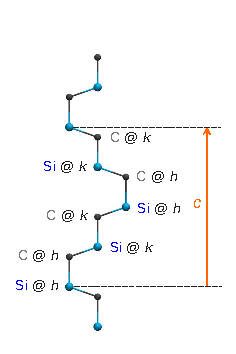
\includegraphics[width=0.38\textwidth]{figures/SiC-non-equiv-sites.pdf}%
        % MAGNETIC MOMENT ELECTRON + SPIN
\begin{tikzpicture}[thick, scale=1.5]
  \def\re{0.3}
  \def\ang{80}
  %\draw[dashed] (\ang-180:2.5*\re) -- (\ang:3.5*\re);
  \draw[mu vector] (0,0) -- (\ang+180:3*\re) node[right] {$\vb*{\mu}_\mathrm{B}$};
  \draw[spin] (0,0) -- (\ang:2.8*\re) node[right] {$\vb{S}$};
  \draw[charge-]
    (0,0) circle (\re) node[scale=1.4] {$-$}
    node[right=0.5] {$\mathrm{e}^-$};
  \draw[->,rotate=\ang-90]
    (0,-0.2*\re)++(-175:{1.6*\re} and {1.3*\re}) arc (-175:-35:{1.6*\re} and {1.3*\re})
    --++ (50:0.3*\re);
\end{tikzpicture}

  % \caption{Schematic of an electron showing magnetic moment and spin.}%
    % \end{center}
\end{wrapfigure}%

In reality the electron is point-like and thus the current loop model is unsuitable. Spin is actually a quantum effect and a consequence of the algebra required to satisfy the Dirac equation of relativistic quantum mechanics. The manifestation of this degree of freedom however has the same dimensionality as $\vec{L}$, allowing us to work with the combination of $\vec{L}$ and $\vec{S}$. 

\begin{wrapfigure}{r}{0.3\textwidth}%
    % \centering%
    \begin{center}
    % 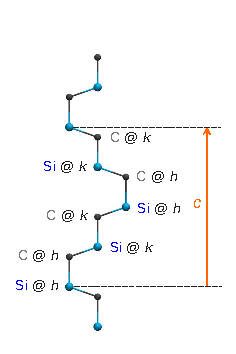
\includegraphics[width=0.38\textwidth]{figures/SiC-non-equiv-sites.pdf}%
        % QUANTUM ANGULAR MOMENTUM - SPIN to scale
\begin{tikzpicture}[thick, scale=1.9] %[z={(0,1)},y={(1,0)},x={(-0.5,0,-0.5)}]
  \def\zmax{1.4}
  \def\s{0.5}
  \def\h{0.8} %1.6/\l
  \def\R{(sqrt(\s*(\s+1))*\h)} % total angular momentum
  \def\M{0.5}
  \def\ang{asin(\M*\h/\R)}
  \def\Rx{sqrt(\R^2-(\M*\h)^2)}
  \def\Ry{0.2*\Rx}
  \coordinate (O) at (0,0);
  
  % AXES
  %\draw[->,thick] (-140:0.005*\zmax) --++ (-140:0.75*\zmax) node[below=-1] {$S_x$};
  \draw[->,thick] (O) --++ (\zmax,0) node[below=-1] {$S_y$};
  \draw[->,thick] (0,-0.9*\zmax) -- (0,\zmax) node[left=-1] {$S_z$};
  
  % CIRCLES
  \draw[Scol!90!black] (0,{\R}) arc (90:-90:{\R}); %,very thin
  %\draw[dashed,myblue] ({\Rx},{\M*\h/sqrt(1+0.2^2)}) arc (0:180:{\Rx} and {\Ry});
  \draw[myblue] (0,-\M*\h) node[left=0,scale=1] {$-\frac{1}{2}\hbar$} --++ ({\Rx},0); %\contour{white}{
  \draw[myblue] (0,+\M*\h) node[left=0,scale=1] {$+\frac{1}{2}\hbar$} --++ ({\Rx},0);
  \draw[spin] (0,0) -- ({\Rx},-\M*\h);
  \draw[spin] (0,0) -- ({\Rx}, \M*\h);
  \node[spin,above right=0] at ({\Rx},{\M*\h}) {$\vb{S}$};
  % \draw[dashed,myblue] ({\Rx},{\M*\h/sqrt(1+0.2^2)}) arc (0:-180:{\Rx} and {\Ry});
  \node[circle, charge-, scale=0.7] (O) {$-$};
  
\end{tikzpicture}

  \caption{Schematic of discrete spin levels.}%
  % \vspace{1em}
\end{center}
\end{wrapfigure}


We thus consider the \index{total angular momentum}{total angular momentum} of a system $J$ given by 
\begin{equation}
    J = L + S 
    \label{eq:total_angular_momentum}
\end{equation}
with $L+S, L+ S - 1, \dots, |L-S|$. 

For a given system with two electrons, combining the individual spin angular momenta, total spin angular momentum 
is the addition of the uncoupled spin operators
\begin{equation}
    \hat{S} = \hat{S}_1 + \hat{S}_2 
    \label{eq:}
\end{equation}
The coupling results in the formation of four spin states with spin quantum number
$S = 0$ and $S = 1$. 
The spin quantum number $S = 0$ leads to a multiplicity of $2S + 1 = 1$, a so called singlet state. 

However, the spin quantum number $S = 1$ results in a multiplicity of
$2S + 1 = 3$, known as triplet states \cite{Piela2014}.  



